 \chapter[Instalación y ejecución de \appName]{Instalación y ejecución\\ de \appName}
\chaptermark{Instalación}

\appName~está distribuido como un \textit{quark} de SuperCollider, es decir, como un conjunto de clases empaquetadas y listas para ser instaladas en el sistema y ser usadas desde \textit{sclang}, el lenguaje de programación de SuperCollider.  Puesto que SuperCollider se distribuye para ser complilado en las plataformas más importantes de escritorio, a saber, Linux, Mac OS y Windows, por la misma razón \appName~ es también multiplataforma. Las instrucciones que aquí se encuentran son comunes a todos los sistemas operativos, si bien, determinadas acciones, como la instalación o la compilación de SuperCollider, pueden variar en sus detalles, para lo cual se ha de acudir a los documentos de ayuda pertinentes en cada caso.

\section{Requisitos}
\begin{description}
	\item[git] Si no está instalado ya en el sistema, ha de ser instalado para poder descargar y manejar los \textit{quarks}: \href{https://git-scm.com/}{\texttt{https://git-scm.com/}}
	
	\item[SuperCollider] Es el programa principal. Contiene tanto el servidor de sonido como el intérprete del lenguaje \textit{sclang}, en el que está escrito \appName. La versión más baja en la que se ha probado que \appName~ funciona es la 3.8. Puede ser compliado desde las fuentes:\\ \href{https://github.com/supercollider/supercollider}{\texttt{https://github.com/supercollider/supercollider}}\\ o desde los binarios ya compilados disponibles:\\ \href{https://supercollider.github.io/download}{\texttt{https://supercollider.github.io/download}}.
	
	\item[sc3-plugins]  Se trata de una colección de \textit{UGens} de SuperCollider mantenidos por la comunidad. Puede ser compilado desde las fuentes:\\ \href{https://github.com/supercollider/sc3-plugins}{\texttt{https://github.com/supercollider/sc3-plugins}} o desde los binarios precompliados para cada sistema operativo desde el mismo repositorio.
\end{description}


\section[Instalación del \textit{quark}\dots]
{Instalación del \textit{quark} de \appName \sectionmark{Instalación del \textit{quark}}}
\sectionmark{Instalación del \textit{quark}}


\appName~ se encuentra alojado en \textit{github}, desde donde pueden ser descargado todo su código fuente. No existen binarios instalables ya que es el propio intérprete de SuperCollider quien se encarga de compilar todas las extensiones y \textit{quarks} instalados en el sistema en cada inicio.

\subsection{Instalación con la interfaz gráfica de \textit{Quark}}

Una vez abierto el editor de SuperCollider, abrir el administrador de \textit{quarks} en el menú \textit{Language}/\textit{Quarks} (fig. \ref{fig:quark_ide}). Buscar en la lista alfabética el \textit{quark} llamado \texttt{SynthiGME}. A continuación, basta con hacer click en el botón con el símbolo <<+>> que hay justo en la columna anterior al nombre. En la parte inferior de la ventana se ofrecen datos relevantes del \textit{quark}, como su origen, una descripción, así como información sobre la instalación. Una vez instalado, es necesario recompilar las clases para poder usarlo, pulsando el botón \textit{Recompile class library}. Con esto \appName~ estará listo para ser utilizado.

\begin{figure}[H]
	\centering
	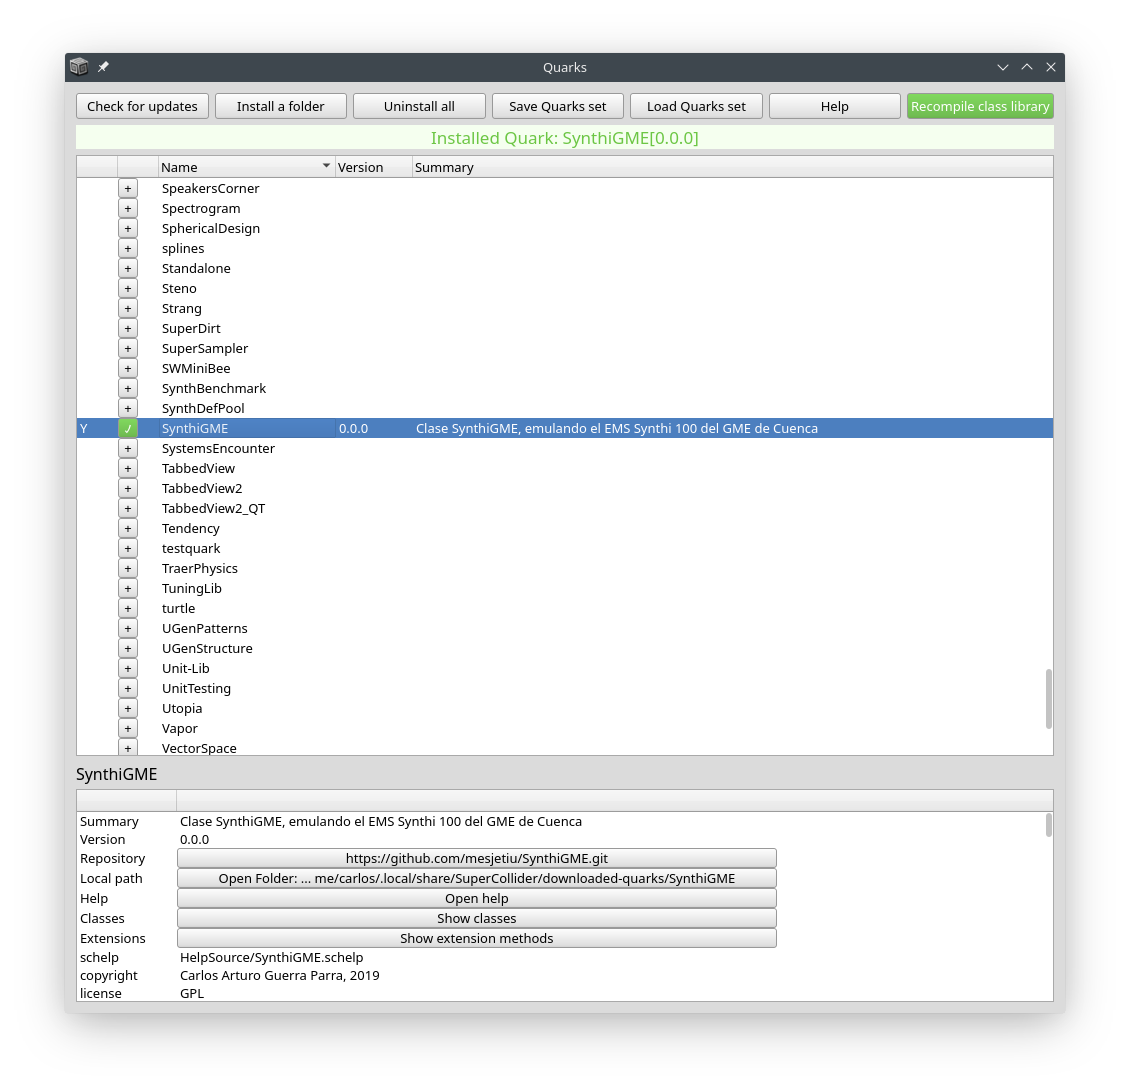
\includegraphics[width=0.7\textwidth]{quark_ide}
	\caption[Instalación gráfica del quark \texttt{SynthiGME}]{Instalación gráfica del quark \textit{SynthiGME}.}
	\label{fig:quark_ide}
\end{figure}


\subsection{Instalación con código}

La forma más sencilla de instalar el \appName~ en su última versión es ejecutando la siguiente línea de código en SuperCollider\footnote{Para ejecutar un código en SuperCollider basta con poner el cursor sobre la línea (o hacer un bloque con las líneas que interesan) y pulsar [Control + Entrar]. Esta combinación podría variar en función del sistema operativo y la versión de SuperCollider, con lo que es conveniente informarse en cada caso.} (Asegurarse de que se tiene conexión a internet):

\begin{lstlisting}[style=SuperCollider-IDE, frame=single, numbers=left]
Quarks.install("SynthiGME");
\end{lstlisting}

SuperCollider buscará en la base de datos de \textit{quarks} y localizará el paquete, que se encuentra en un repositorio de \textit{Github}\footnote{\href{https://github.com/mesjetiu/SynthiGME.git}{\texttt{https://github.com/mesjetiu/SynthiGME.git}}}. Si todo ha ido bien, se verá la siguiente salida en \textit{Post window}:

\begin{lstlisting}[frame=single, numbers=left]
-> Quarks
Installing SynthiGME
Adding path: /[user path]/.local/share/SuperCollider/downloaded-quarks/SynthiGME
SynthiGME installed
-> Quark: SynthiGME[0.0.0]
\end{lstlisting}

En la última línea aparecerá entre corchetes la versión de \appName~ instalada, que coincidirá con la última \textit{release} en la rama \textit{master} del repositorio de la aplicación.

Una vez instalado, es necesario recompilar todas las clases para poder usar las del \textit{quark} recién instalado. Ello se puede hacer con la combinación [Control+Mayúsculas+L]\footnote{Esta combinación funciona en Linux, pero podría variar en función del sistema operativo o de la versión de SuperCollider.} o ejecutando el siguiente código:

\begin{lstlisting}[style=SuperCollider-IDE, frame=single]
thisProcess.recompile;
\end{lstlisting}


\section{Ejecutar \appName}
\label{ejecucion}

\appName~ es, en esencia, un conjunto de clases, de entre las cuales, solo una está diseñada para ser instanciada por el usuario: \texttt{SynthiGME}. Esta clase contiene el método \texttt{run}, que pone en marcha todas las rutinas de arranque de la aplicación: crea los \textit{busses} de audio que comunican todos los módulos entre sí, todos los \texttt{Synths}, o <<sintetizadores>> de SuperCollider, las rutinas, etc. Configura el servidor de audio para que acepte el número adecuado de entradas y salidas requerido.

El siguiente código muestra varias formas de ejecutar \appName:
\begin{lstlisting}[style=SuperCollider-IDE, frame=single,  numbers=left]
// Se instancia la clase SynthiGME
// y se ejecuta su método "run":
~synthi = SynthiGME();
~synthi.run();

// o, ambas sentencias en una:
~synthi = SynthiGME().run;

// Al introducir el objeto en una variable, podemos cerrar el programa ejecutando el método "close":
~synthi.close;
\end{lstlisting}

Si todo el proceso se ha producido satisfactoriamente, \textit{Post window} mostrará una salida similar a esta:

\begin{lstlisting}[frame=single, numbers=left]
Conexión de salida stereo canales 1 a 8...OK
Conexión de salida stereo canales 1 a 4...OK
Conexión de salida stereo canales 5 a 8...OK
Conexión de salida de cada canal individual...OK
Output Channels...OK
Filters...OK
Octave Filter Bank...OK
Ring Modulators...OK
Echo A.D.L...OK
Noise Generators...OK
Random Voltage Generator...OK
Slew Limiters...OK
Oscillators...OK
Envelope Shapers...OK
Input Amplifier Level...OK
Conexiones en Patchbay de audio...OK
Conexiones en Patchbay de voltage...OK
Conexión de entrada Input Amplifiers, canales 1 a 8 a puertos de SC...OK
SynthiGME en ejecución
\end{lstlisting}



Es importante notar que el proceso de arranque reiniciará automáticamente el servidor de sonido para asegurar que todos los cambios en la configuración surten efecto. Esto significa que si se requiere ejecutar más código de SuperCollider simultáneamente, este ha de ser ejecutado después que \appName. 

En pocos segundos se abrirán 7 ventanas ordenadas y adaptadas al tamaño de la pantalla, representando a los 7 paneles del Synthi 100 del GME de Cuenca. A partir de aquí, si \textit{Post window} no señala ningún error o mal funcionamiento en la ejecución, el programa ya está listo para ser usado.




